\section{Time box 2}
\subsection{Time box planning}
Show meeting in week 11.
\subsubsection{Work to be done in this time box}
\begin{itemize}
	\item ARM to FPGA interface
	\begin{itemize}
		\item Mount
		\item Test
	\end{itemize}
	\item PLC module
	\begin{itemize}
		\item Mount x7
		\item Test
	\end{itemize}
	\item Daemon
	\item Power switch
	\begin{itemize}
		\item Block diagram
	\end{itemize}
	\item Module design
\end{itemize}
\paragraph{Description:}
\begin{description}
	\item[ARM to FPGA interface] The connection between the ARM7 CPU and the FPGA board, has to be mounted, tested and debugged.
	\item[PLC module] The powerline module has to be mounted 7 times for all the groups, tested and debugged.
	\item[Daemon] 
	\item[Power switch] Block diagram of the power switch, which shall activate the different modules connected to it (wind-turbine, photo-voltaic cells etc.) and control the current flow.
	\item[Module design]
\end{description}

\subsection{ARM to FPGA interface}



\subsection{PLC module}
The second version of the Power line module was decreased size, which lead to problems when making the PCB, as a lot of tracks short-circuited. A third version has been made, which has larger clearance between the tracks and the ground plane. The PCB has been mounted and tested, which is describe in the \textit{EPRO 3 \& 4 PLC - Hardware Interface} report. As a short resume, the communication between two boards through power line works without reading any invalid characters (test period of 15 min.). The 5 volt power supply has been tester to withstand at minimum 2.4 Amp. where a voltage drop of approximately 0.1Volt was observed. 
A single error has been found which is corrected before ordering and mounting the 6 PLC boards needed (one for each module in the system/group).

\begin{figure}[H]
	\begin{centering}
		 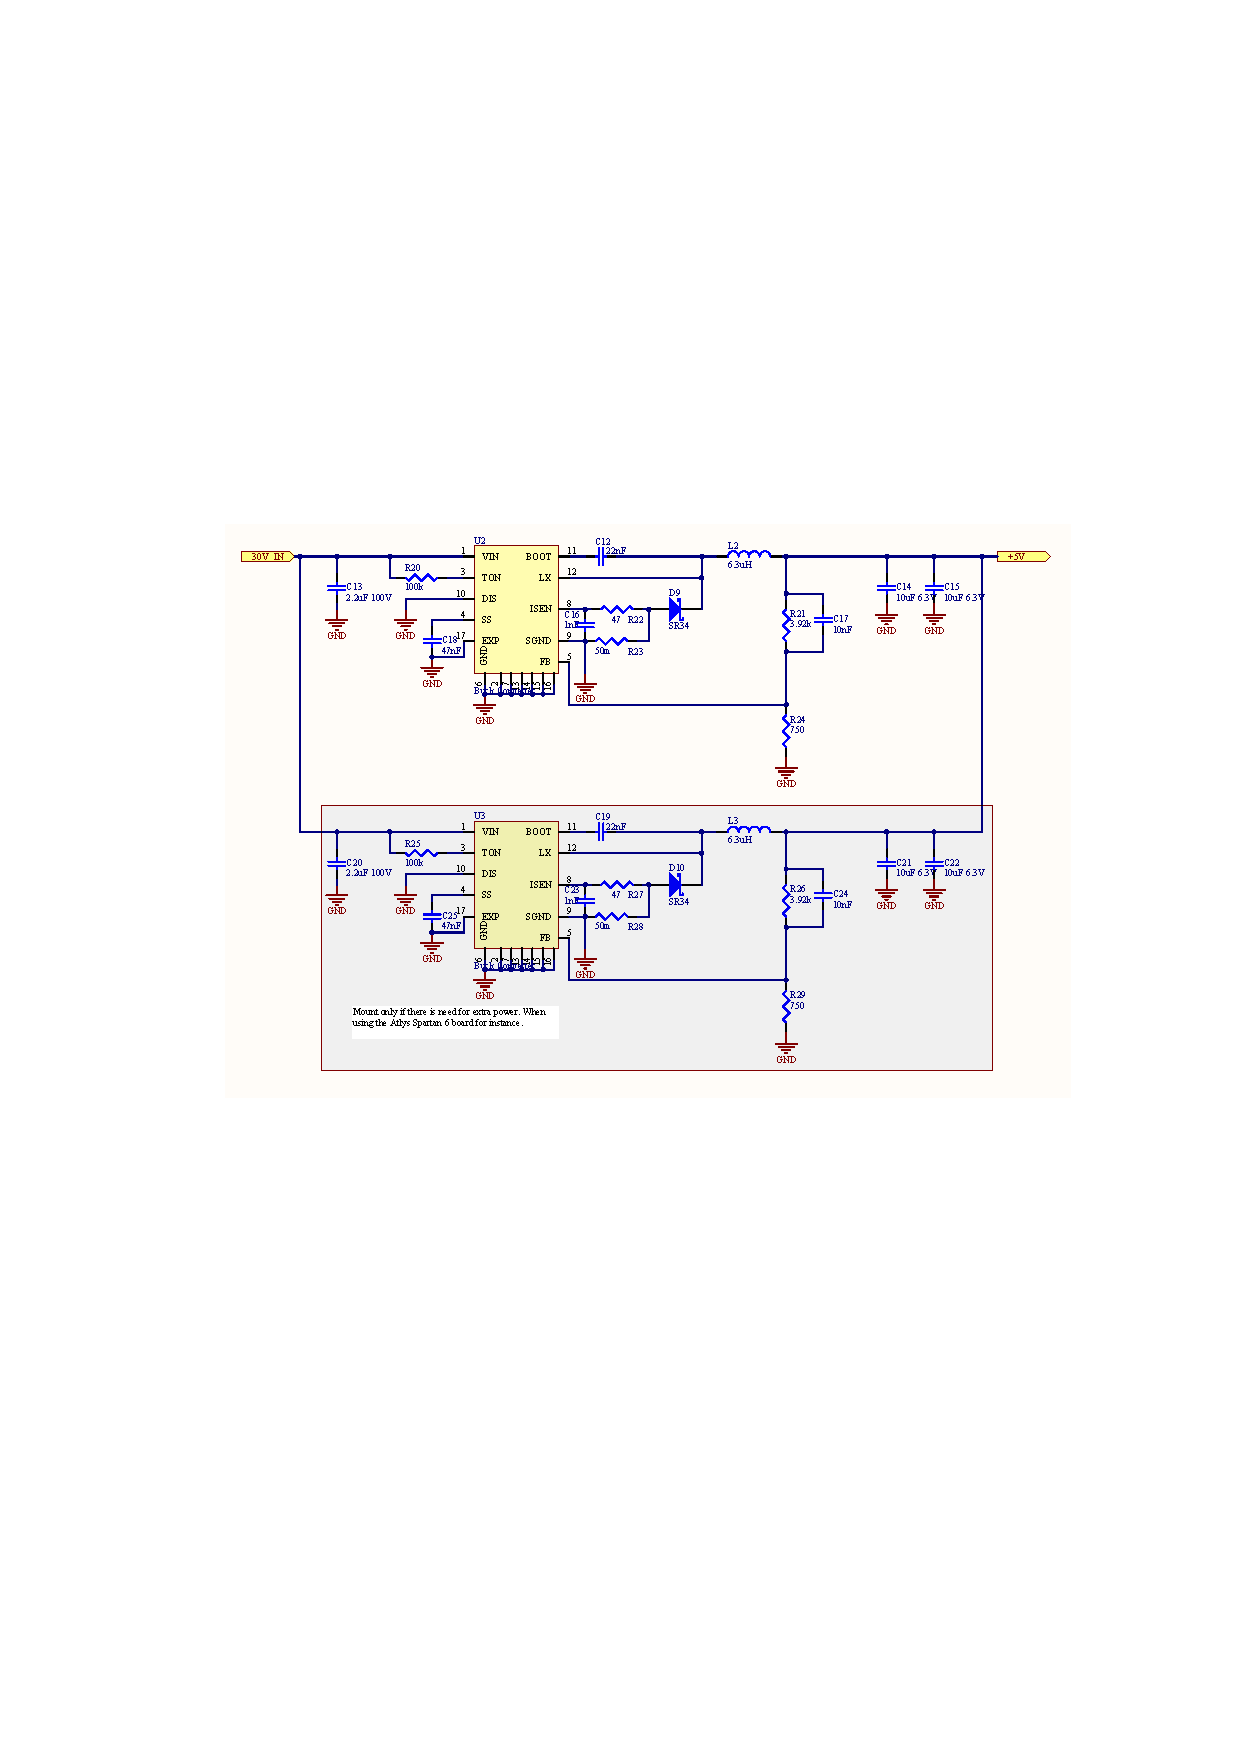
\includegraphics[width=0.9\textwidth,page=1,angle=0]{images/SIG60_v0_4}
		\caption{Power line circuit version 0.4}
	\end{centering}
\end{figure}

\begin{figure}[H]
	\begin{centering}
		 \includegraphics[width=0.8\textwidth,page=2,angle=0]{images/SIG60_v0_4}
		\caption{Power supply. 2 x 5 volt 3 ampere version 0.4.}
	\end{centering}
\end{figure}

\begin{figure}[H]
	\begin{centering}
		 \includegraphics[width=0.8\textwidth,page=3,angle=0]{images/SIG60_v0_4}
		\caption{PCB layout of the power line circuit and the 5 volt power supply version 0.4.}
	\end{centering}
\end{figure}


\subsection{Daemon}
\begin{itemize}
	\item Overview
	\item Make daemon to run on uClinux
	\item The rc file (startup file)
	\begin{itemize}
		\item Configure network
		\item Start daemon as background process
	\end{itemize}
\end{itemize}


\subsection{Power switch}
The power switch is the part of the hub that traffics the current from and to its connected modules. 
\\ Inspiration: 
\url{http://www.pwrhub.com/}
\\ \url{http://www.linear.com/product/LTC4357}
\\ \url{http://cds.linear.com/docs/Demo\%20Board\%20Manual/dc1203A.pdf} demo board.
\\ Power Mosfets:
\url{http://pdf1.alldatasheet.com/datasheet-pdf/view/234175/IRF/IRFP4468PBF.html}
\\ Power rectifiers
\url{http://pdf1.alldatasheet.com/datasheet-pdf/view/172142/ONSEMI/MBR60H100CT.html}


\subsection{Module design}


